\documentclass{standalone}
\usepackage{tikz}
\usetikzlibrary{positioning,arrows.meta,shapes.misc,calc}

% COLORS
\usepackage{xcolor}
\colorlet{myred}{red!80!black}
\colorlet{myblue}{blue!80!black}
\colorlet{mybluee}{myblue!80!black}
\colorlet{mygreen}{green!60!black}
\colorlet{myorange}{orange!70!red!60!black}
\colorlet{mydarkred}{red!30!black}
\colorlet{mydarkblue}{blue!40!black}
\colorlet{mydarkgreen}{green!30!black}
\definecolor{mygray}{HTML}{D1D2D4}

\begin{document}
\begin{tikzpicture}[
    >=Stealth,
    block/.style={rectangle, rounded corners,  align=center},
]

% Placeholder image
\node[inner sep=0, outer sep=0] (image) at (0,0) {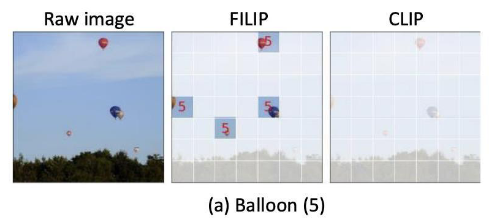
\includegraphics[width=7cm,height=3cm]{tikz/chapter11 - FILIP vs CLIP.png}};
\node[fill=white, xshift=0cm, yshift=1.35cm] {\footnotesize FILIP};
\node[fill=white, xshift=2.3cm, yshift=1.35cm] {\footnotesize CLIP};
\node[fill=white, xshift=-2.2cm, yshift=1.35cm] {\footnotesize Raw Image};
\node[fill=white, xshift=1cm, yshift=-1.35cm, minimum height = 0.5cm, minimum width = 2cm] {};
\node[fill=white, xshift=0cm, yshift=-1.35cm] {(Balloon Class)};
\end{tikzpicture}

\end{document}